\documentclass[../../ClassicThesis.tex]{subfiles}
\begin{document}

\note{cross-platform/ headless capabilites chapter missing - then we
  can introduce the separated client/ server package in the platener
  chaper}

\section{Convertify}
\label{sec:framework-convertify}

In this section we present {\convertify}, a web-framework for working
with {\threedmodel}s. {\convertify} consists of three code packages: a
frontend package, a backend package and a common package.
Figure~\ref{fig:platener-package-diagram-overivew} shows a package
diagram. The common package provides utilities that can be used by
frontend and backend applications. Such utilities are maths helpers or
the plugin manager. Secondly, there are two packages which integrate
with either frontend or backend applications that use {\convertify}.
The frontend package contains components for rendering and scene
management. The backend packages provides similar components, which
work without a DOM-tree. Thus, backend packages can be run in
{\nodejs} and do not require a browser environment, see
Section~\ref{sec:convertify-is-isomorphic}. The plugins package and
the client package are not part of the {\convertify} framework. These
packages are implemented by an application like {\platener}, which is
based on {\convertify}. The plugins package provides an exchangeable
set of features. A plugin interacts with the scene and its
{\threedmodel}s via lifecycle events. The client package gives the
look and feel of the application. This package contains frontend
components. The client wires up the {\userinterface} and the
computation logic.

\begin{figure}[h]
  \centering
  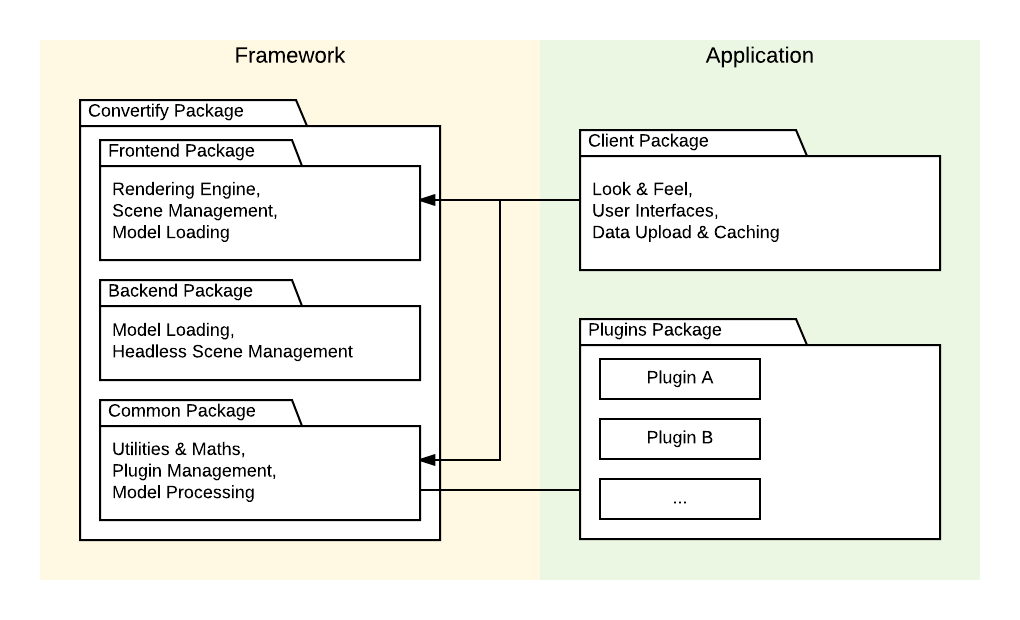
\includegraphics[width=1\textwidth]{03-architecture-package-diagram-overview}
  \caption{Packages of {\convertify}}
  \label{fig:platener-package-diagram-overview}
\end{figure}

We will explain core features of {\convertify} in
Section~\ref{sec:convertify-core-features}. Then we will dive into
its plugin system in Section~\ref{sec:plugin-system}. {\convertify} is
based on previous work by \citeauthor{bachelor-thesis}. We will give a
short comparison of their work with {\convertify} in
Section~\ref{sec:brickify-comparison}. We elaborate on the client
package when we talk about our application {\platener} in
Section~\ref{sec:application-platener}.

\subsection{Introduction to the Core System of {\convertify}}
\label{sec:convertify-core-features}

In this section we present the core system of {\convertify}.
{\convertify} helps to build WebGL applications by providing
abstractions to the rendering engine and by composing
features into plugins. We will focus on important design
decisions, which are scene management, rendering and
plugins.

\subsubsection{{\threedmodel}s Are Managed in a Flat Scene
  Graph}

A flat scene graph is a scene graph with only one level of
hierarchy. Thus, our entities in the scene graph do not have
any children. We only need a flat scene graph, because we
only have to manage and access the input models.

We implement the flat scene graph using \class{Nodes}.
\class{Nodes} are abstract objects, which represent an
entity in our scene graph. Each \class{Node} references an
input model and transforms. The input model is a
face-vertex-mesh, that is either used for rendering or used
by algorithms for further computation. Transforms
describe spatial properties like position, scale or
rotation.

All \class{Nodes} are part of a \class{Scene}. A
\class{Scene} holds references of \class{Nodes}, so we can
access the input models for later usage. \class{Nodes} are
added to or removed from the \class{Scene} via the
\class{SceneManager}. Figure~\ref{fig:scene-graph} shows how
these classes relate.

\begin{figure}[h]
  \centering
  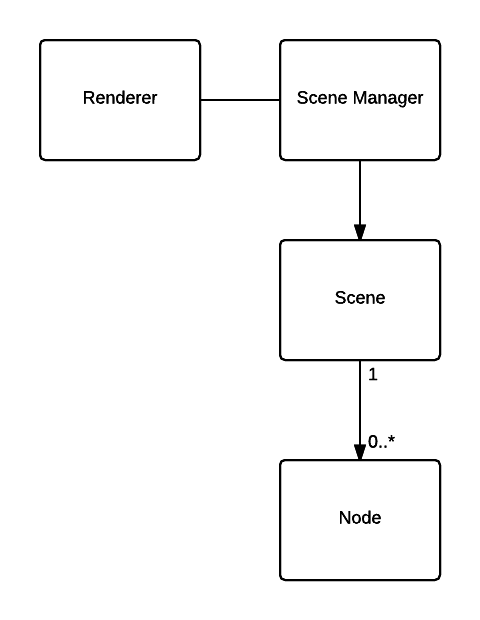
\includegraphics[width=0.6\textwidth]{03-architecture-scene-graph}
  \caption{Relation of scene graph components}
  \label{fig:scene-graph}
\end{figure}

\subsubsection{{\threedobject}s Are Rendered with
  {\threejs}}

% A \class{Scene} contains all \class{Nodes} that reference an
% input model.
Though \class{Nodes} represent entities in the scene of
{\convertify}, only {\threejs} objects can actually be
rendered. Such {\threejs} objects are instances of
\class{THREE.Object3D}\footnote{\url{http://threejs.org/docs/\#Reference/Core/Object3D}}.
This is a generic object, which can be rendered into a WebGL
scene. These \class{THREE.Object3D} will be displayed on the
screen. The scene graph of {\threejs} is not flat. A
\class{THREE.Object3D} can have a hierarchy of objects of
any size. Figure~\ref{fig:nodes-and-three} shows the
\class{THREE.Object3D} in the context of \class{Nodes} and
the \class{Renderer}.

We use a \class{Renderer} instance to bring {\threejs} entities to the
screen. The \class{Renderer} sets up a WebGL context and initializes
{\threejs}. In {\convertify} we use plugins, in which we can provide
additional features. Plugins are described in detail in
Section~\ref{convertify-emits-events}. We associate each plugin with a
\class{THREE.Object3D} and vice-versa. Thus, we enable plugins to
enhance the scene with new objects. The \class{Renderer} then
traverses the hierarchy of each associated \class{THREE.Object3D} and
renders it.

A plugin accesses \class{Nodes} via system events. We explain system
events in Section~\ref{convertify-emits-events}. The \class{Node}
contains the input model. The plugin uses the \class{Node} to append
data to its associated \class{THREE.Object3D}. The \class{Node}
transforms are thereby applied to the {\threejs} entities.


\begin{figure}[h]
  \centering
  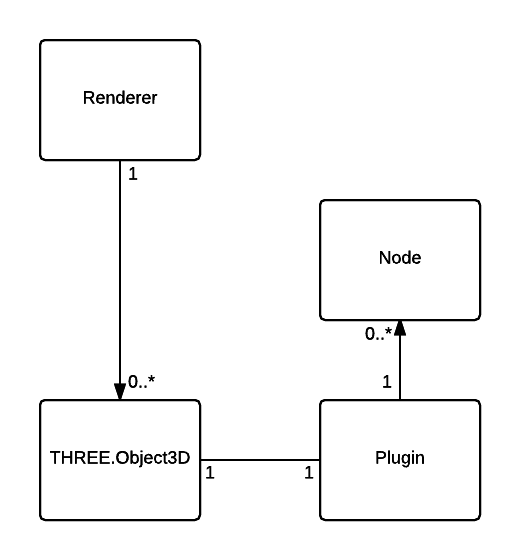
\includegraphics[width=0.6\textwidth]{03-architecture-threejs-objects}
  \caption{\class{Nodes} and indirectly associated \class{THREE.Object3D}}
  \label{fig:nodes-and-three}
\end{figure}

\subsubsection{Convertify Emits System Events}
\label{convertify-emits-events}

During the loading and render process, {\convertify} emits system
events. A system event notifies subscribers about changes of the state
of {\convertify} during its lifecycle. Such changes can be touch or
pointer interactions with rendered models in the scene
(\name{onPointerEvent}) or change events to the scene graph
(\name{onNodeAdd}, \name{onNodeRemove}). Figure~\ref{fig:lifecycle} shows
the full lifecycle and event loop of {\convertify}. Events concerning
the scene management will have the \class{Node} as payload. Thus,
other system components can access the \class{Node}.

\begin{figure}[h]
  \centering
  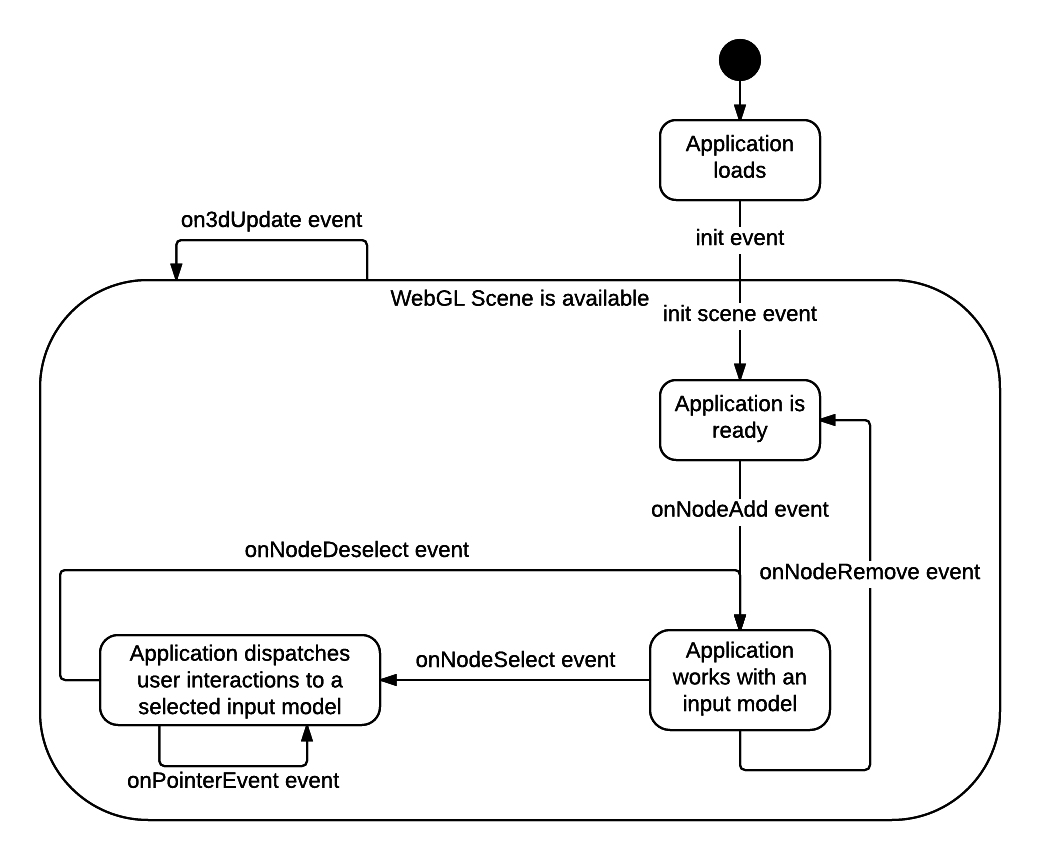
\includegraphics[width=1.2\textwidth]{03-architecture-lifecycle-convertify}
  \caption{The complete lifecycle of {\convertify}}
  \label{fig:lifecycle}
\end{figure}

\subsubsection{{\convertify} Integrates Additional Features
  Via Plugins}

{\convertify} loads additional features into its system via
\class{Plugins}. \class{Plugins} encourage to decompose
feature sets into independent components. A \class{Plugin}
is a separate code package, that adds features for the WebGL
scene or algorithmic computation units. Therefore, it
provides a set of methods which can be called upon emitted
system events. We refer to these callbacks as
\class{PluginHooks} or simply hooks. We will look at the
details of \class{Plugins} and plugin communication in
Section~\ref{sec:plugin-system}.


% User
% interfaces are implemented within the same code package.
% This does not separate the web-interface from the scene
% features. Thus, it is hard to observe and apply changes to
% the system. The interface code uses a \class{Bundle} as an
% entry point to the plugin and scene system. The
% \class{Bundle} starts \class{Plugins} and loads
% {\threedmodels} from the filesystem into the application.

% {\brickify} provides abstractions for scene management and
% rendering. Plugins interact with the internal system via
% hooks. The separation of {\lego}-conversion features from
% the rendering engine bring clear interfaces. We encountered
% several hick-ups with this architecture when we tried to
% organize the communication between several plugins. In the
% following sections, we outline our improvements to the
% internal system of {\brickify}. In
% Section~\ref{sec:reuses-brickify} we talk about components
% which could be reused with minor adaptions.
% Section~\ref{sec:plugin-system} presents the necessary
% changes to the plugin system.

% The framework {\convertify} is based on the application
% {\brickify} by \citeauthor{brickify-thesis}. {\brickify}
% provides features like rendering or the scene graph, which
% are use by {\convertify}.


% \subsection{The Framework is Based on Brickify}
% \label{sec:based-brickify}

% \note{refromulate this section into a related work section}
% \note{then put all details from the chapter into the next
%   section, where we explain how convertify actually works}

% The framework {\convertify} is based on the application {\brickify}
% by \citeauthor{brickify-thesis}. {\brickify} is a web-application
% which converts {\threedmodel}s into a hybrid model, consisting of
% {\lego} bricks and fewer 3D-printable parts. The previous work
% provides features like rendering or scene graphs, which can be
% shared with {\convertify}. In this section we present important
% design decisions of {\brickify}, which will help understanding how
% our framework
% works.

% {\brickify} implements a flat scene graph using \class{Nodes}. Each
% \class{Node} references an input model, has a {\threejs} object and
% transforms. The {\threejs} object is a \class{THREE.Object3D}. This
% is a generic object, which can be rendered into a WebGL scene with
% {\threejs}. This \class{THREE.Object3D} will be displayed on the
% screen by {\brickify}. The transforms describe spatial properties
% like position, scale or rotation and are applied to the {\threejs}
% node. Note, that \class{Nodes} represent entities in the scene, but
% only {\threejs} nodes can actually be rendered.

% \note{introduce the terms more smoothly. also what is a
%   scene graph in this context?}

% The \class{Nodes} are part of a \class{Scene}. The \class{Renderer}
% sets up a WebGL context and initializes {\threejs}. Then the
% \class{SceneManager} passes all active \class{Scenes} to the
% \class{Renderer}, which will traverse the scene graph and
% render each attached \class{THREE.Object3D}.
% Figure~\ref{fig:scene-graph} shows how these classes interact.
% During that loading and render process, {\brickify} emits system
% events, e.g. change events to the scene graph (\textit{onNodeAdd},
% \textit{onNodeRemove}).

% \note{FIGURE: look up how interactions really are! maybe
%   show emission of events also, maybe class diagram is not
%   suitable?}

% \begin{figure}[h]
%   \centering
%   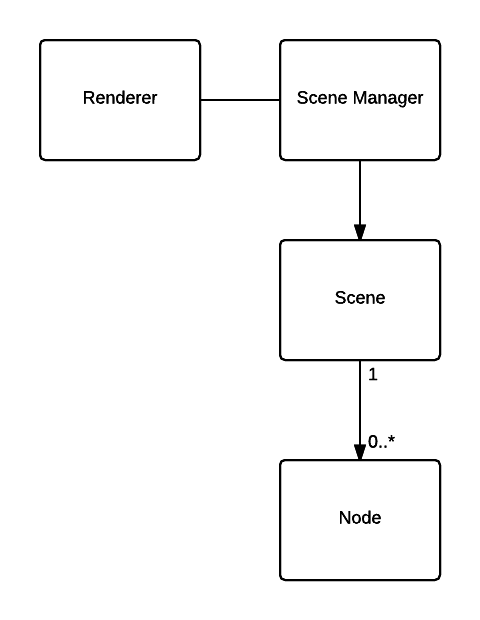
\includegraphics[width=0.6\textwidth]{03-architecture-scene-graph}
%   \caption{Interaction of scene graph components.}
%   \label{fig:scene-graph}
% \end{figure}

% {\brickify} decomposes its features into \class{Plugins}. A
% \class{Plugin} provides a set of methods which can be called upon
% emitted system events to interact with the WebGL scene.
% \citeauthor{brickify-thesis} refers to these callbacks as
% \class{PluginHooks} or just hooks.

% \note{what is a bundle doing here, better intro}
% User interfaces are implemented within the same code package. This
% does not separate the web-interface from the scene features. Thus, it
% is hard to observe and apply changes to the system. The
% interface code uses a \class{Bundle} as an entry point to the plugin
% and scene system. The \class{Bundle} starts \class{Plugins} and loads
% {\threedmodels} from the filesystem into the application.

% {\brickify} provides abstractions for scene management and rendering.
% Plugins interact with the internal system via hooks. The separation of
% {\lego}-conversion features from the rendering engine bring clear
% interfaces. We encountered several hick-ups with this architecture
% when we tried to organize the communication between several plugins.
% In the following sections, we outline our improvements to the internal
% system of {\brickify}. In Section~\ref{sec:reuses-brickify} we talk
% about components which could be reused with minor adaptions.
% Section~\ref{sec:plugin-system} presents the necessary changes to the
% plugin system.

% \subsection{The Framework Reuses Ideas and Components of Brickify}
% \label{sec:reuses-brickify}

% {\brickify} provides a set of core feature any WebGL application can
% make use of. This includes components like the render loop, scene
% management and plugin loading. {\convertify} has the goal to provide
% these essential components to help implementing WebGL application
% fast-forwardly. The implementation of such applications should be
% independent from any user interface code or required frontend
% libraries, avoiding additional vendor-locks to {\threejs}. In this
% section we explain, how we reached this goal.

% \myNotes{work on that section}
% re-uses render loop, scene management, plugin loading, bundle

% changes were: in project structure and ui code <> lots of mixing with
% ui code (convertify does not have any ui code out of the box. that
% will be part of the application that uses convertify)

% To make {\convertify} a multi-purpose WebGL framework, we stripped
% away any interwoven interface code from the \class{Renderer},
% \class{SceneManager} and \class{Bundle}. We also used the plugin
% system of {\brickify}. The applied changes to the plugin system are
% described in the following section.

\subsection{{\convertify} Provides a Plugin System}
\label{sec:plugin-system}

% - Subsection overview

In this section, we present a plugin system that reacts to
{\convertify}'s system events. Additionally, we present a
method, which organizes communication between
\class{Plugins}.

% - Plugin definition in Convertify
% - *feature for web gl scene and reaction on changes of the scene*
% - *full fledged applications will implement a set of plugins to
% provide functionality and web-ui code to provide interface*

A \class{Plugin} bundles an exchangeable set of features which will
interact with the WebGL scene or will react on changes to the scene.
Such features are touch interactions with the rendered model or
computation on the model data when a \class{Node} is added to the
scene. Any full fledged application implements a set of
\class{Plugins} to provide the scene functionality. E.g. a concrete
conversion strategy provided by {\platener} is implemented by a single
\class{Plugin}, the \name{PlatenerPipeline} plugin.
Figure~\ref{fig:plugin-constellation} shows our seven plugins and how
they relate to each other. We give an overview for each plugin in
Section~\ref{sec:platener-uses-plugins}.

\begin{figure}[h]
  \centering
  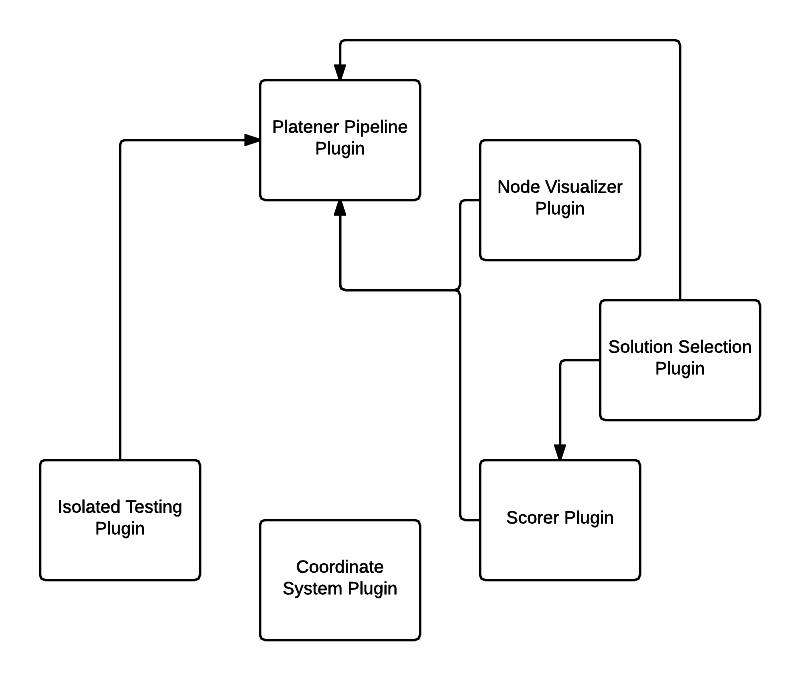
\includegraphics[width=1\textwidth]{03-architecture-plugin-constellation}
  \caption{Platener's plugins and their dependencies.}
  \label{fig:plugin-constellation}
\end{figure}

\subsubsection{Plugins Interact with the Internal System via
  Lifecycle Events}

% - needs-ref :: Lifecycle events in Convertify (= PluginHooks of
% Brickify, Convertify vs. Plugins)
% - needs-figure :: Example Plugin, interacting via PluginHooks
% - System dispatches events (where do events come from?)

{\convertify} emits system events from internal components.
Figure~\ref{fig:lifecycle} depicts the system's lifecycle
and the emitted events. The subscribers to system events are
\class{Plugins}. Each event can be handled by a
\class{PluginHook}, if a \class{Plugin} implements it. To
implement a \class{PluginHook} each \class{Plugin} registers
a callback for that event. These callbacks get called when
the event is dispatched by the system. Thus, \class{Plugins}
can react to each event and apply their own functionality to
the scene or even the model geometry. With this we emphasize
compact computation units in plugins, which can still
interact freely with the system.

To better illustrate the work flow of plugins, we have a look at the
\name{PlatenerPipeline} plugin. The \name{PlatenerPipeline} plugin is
a \class{Plugin} implemented for {\platener}. The \class{Plugin} reads
the model data from a \class{Node} after a {\threedmodel} was loaded
into the scene. Then it processes the data to create a {\lasercutter}
conversion. When the model is deleted from the scene by a user, the
plugin releases the processed data. This plugin does not react to
further user interactions, like clicking or rotating the model.
Figure~\ref{fig:workflow-platener-pipeline} shows how this plugin
integrates with {\convertify} events.

\begin{figure}[h]
  \centering
  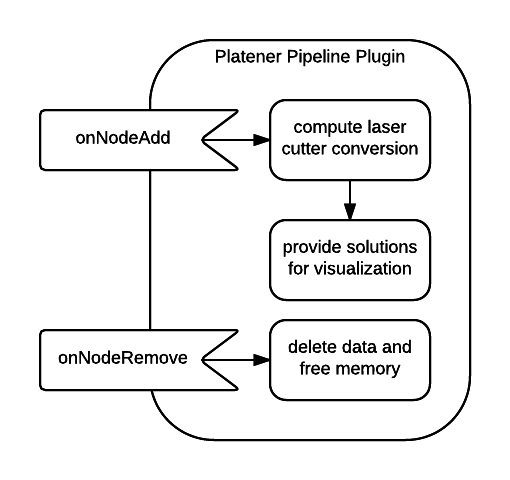
\includegraphics[width=0.6\textwidth]{03-architecture-platener-pipeline}
  \caption{Workflow of the \name{PlatenerPipeline} plugin.}
  \label{fig:workflow-platener-pipeline}
\end{figure}

\subsubsection{Organizing Plugin Communication with a
  Dispatcher}

% - needs-ref :: mediator organizes communication
% - needs-figure :: mediator between dispatched system events and
%                   plugins (internal handling of system events
%                   before reaching plugins)

As {\convertify} manages multiple plugins, which either represent
computation logic or render components, we have to know exactly when
each of these plugins will interact with the system. As
Figure~\ref{fig:plugin-constellation} shows, the dependencies between
plugins are hard to oversee. We propose a \class{Dispatcher}
component, behaving similar to the \name{mediator} pattern.
Figure~\ref{fig:plugin-constellation-with-dispatcher} shows how the
dependencies between plugins are managed with a \class{Dispatcher}.

\begin{figure}[h]
  \centering
  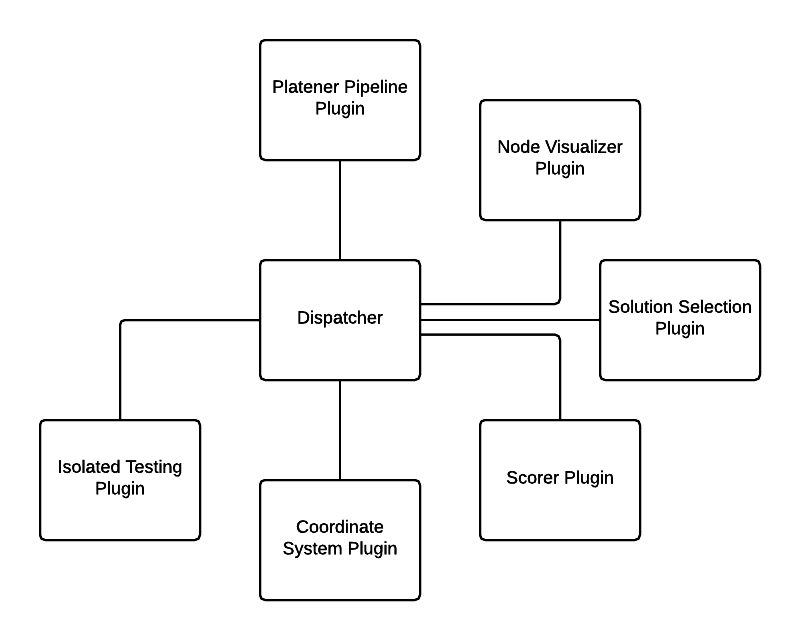
\includegraphics[width=1\textwidth]{03-architecture-plugin-constellation-with-dispatcher}
  \caption{Platener's plugins, managed by a \class{Dispatcher}.}
  \label{fig:plugin-constellation-with-dispatcher}
\end{figure}

According to \citeauthor{gof}, the \name{mediator} pattern is a
behavioral software design pattern. The mediator encapsulates
interconnections of components. It acts as a communication hub and
coordinates its clients. The client components are loosely coupled as
the clients communicate with the mediator instead of communicating
with each other directly. With a mediator we can model many-to-many
relationships \cite[p. 273]{gof}.
% https://sourcemaking.com/design_patterns/mediator


The \class{Dispatcher} implements every \class{PluginHook}. All system
events are emitted to the \class{Dispatcher} first, before the
\class{Dispatcher} will remit them to the \class{Plugins}, see
Figure~\ref{fig:dispatching-events}. In our case the
\class{Dispatcher} is the mediator, where as the \class{Plugins} are
the mediator's clients. With this component in the middle, we can
control the order in which the events will be received by the
\class{Plugins}. We have to determine the order of \class{PluginHook}
executions explicitly, because for different events, different
\class{Plugins} have to run first. E.g. {\platener} wants to process
the model data before it is rendered when a user adds a node to the
scene. But it wants to destroy the visualization before releasing all
the computed data. We cannot solve this problem, by dispatching all
events to all plugins in the same order.

\begin{figure}[h]
  \centering
  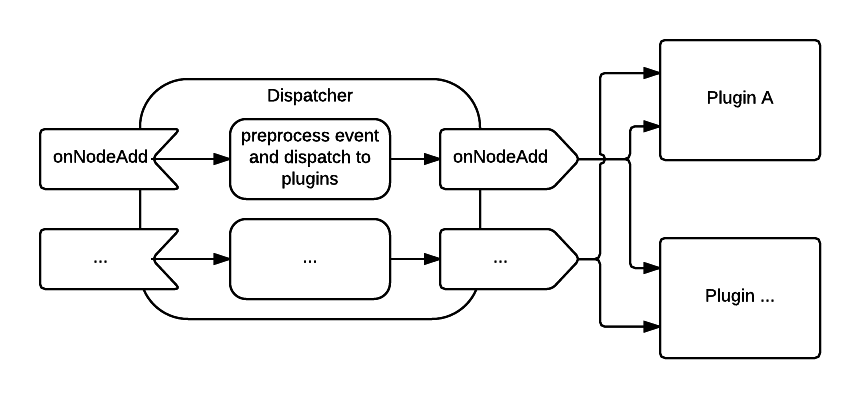
\includegraphics[width=1\textwidth]{03-architecture-dispatching-events}
  \caption{The \class{Dispatcher} remits system events in an explicit order.}
  \label{fig:dispatching-events}
\end{figure}

To model many-to-many relationships between \class{Plugins} and
\class{Plugins}, we enhance the \class{Dispatcher} with
\class{Protocols}. A \class{Protocol} is a mixin implemented by the
\class{Dispatcher}. A mixin adds functionality to an object by object
composition\cite[p.~81]{js-design-patterns}. In {\javascript}
we realize this with meta-programming. The \class{Protocol} then
delegates functionality from the \class{Dispatcher} to a
\class{Plugin}.
% \class{Protocols} define mixins on the
% \class{Dispatcher} which allow delegation of functionality from the
% \class{Dispatcher} to a \class{Plugin}.
The delegation pattern achieves the results of multiple inheritance by
object composition. The delegation pattern speaks of delegating
objects and delegates. A delegating object calls external
functionality on a delegate object, which is available through a
predefined interface \cite{delegation-pattern}. In our case, the
\class{Dispatcher} is the delegating object and the \class{Plugin} is
the delegate. The \class{Protocol} helps to define the interface
between the \class{Dispatcher} and a \class{Plugin}. Two
\class{Plugins} now communicate with each other via the
\class{Dispatcher}. One \class{Plugin} calls functionality on the
\class{Dispatcher} which was exposed by a \class{Protocol}. The
\class{Protocol} ensures that the \class{Dispatcher} delegates an
action to another \class{Plugin}. Figure~\ref{fig:protocol-and-plugin}
shows how the mediator connects two \class{Plugins}.
% http://best-practice-software-engineering.ifs.tuwien.ac.at/patterns/delegation.html
% https://developer.apple.com/library/ios/documentation/General/Conceptual/DevPedia-CocoaCore/Delegation.html

\begin{figure}[h]
  \centering
  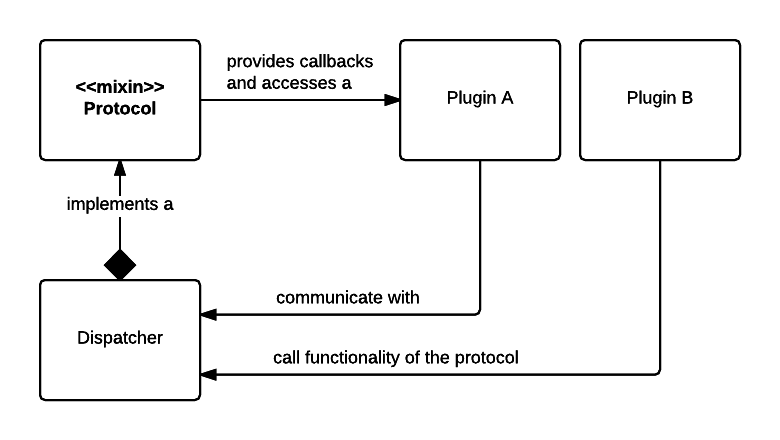
\includegraphics[width=1\textwidth]{03-architecture-protocol-and-plugin}
  \caption{Plugin~B can use features of Plugin~A by calling functionality of the \class{Protocol} implemented by the \class{Dispatcher}.}
  \label{fig:protocol-and-plugin}
\end{figure}

When applications grow, it is hard to observe all messaging between
components at once. With the \class{Dispatcher}, we wire up all
communication with \class{Plugins} in one place. Due to explicit
ordering of callback executions, we have fine-grained control for each
\class{Plugin}. \class{Protocols} define clean interfaces for
inter-\class{Plugin} communication.

% Each application implemented with
% the {\convertify} framework has to implement a custom
% \class{Dispatcher}.

% - *full fledged applications will implement a mediator to organize
% feature communication*

\subsubsection{A \class{Bundle} Is the Entry Point for Applications Using {\convertify}}
\label{sec:bundle-entry-point}

{\convertify} provides a \class{Bundle} instance for its frontend and
backend packages. A \class{Bundle} is the entry point for
applications, that use {\convertify}. E.g {\platener} accesses the
\class{Bundle} of the frontend package to initialize the web app with
{\convertify}'s WebGL scene. The \class{Bundle} is a controller for
{\convertify}. It loads models into the system and exposes controls
for the scene. With this, we can animate the scene programmatically or
sync the scenes of multiple {\convertify} instances. We need a bundle
for both, frontend and backend package, because data access is done
differently in browser environments and {\nodejs}.

In the preceding section, we introduced a \class{Dispatcher}, which
organizes the communication between plugins and {\convertify}. As
{\convertify} is a framework, multiple applications can be realized
with it. Now, every application wants to organize its plugins and
event handlers differently. That is why, each application implements
its own \class{Dispatcher} instance. The \class{Bundle} can be
configured with such a \class{Dispatcher}.
Figure~\ref{fig:bundle-dispatcher} shows how the \class{Bundle} in the
context of an application.

\begin{figure}
  \centering
  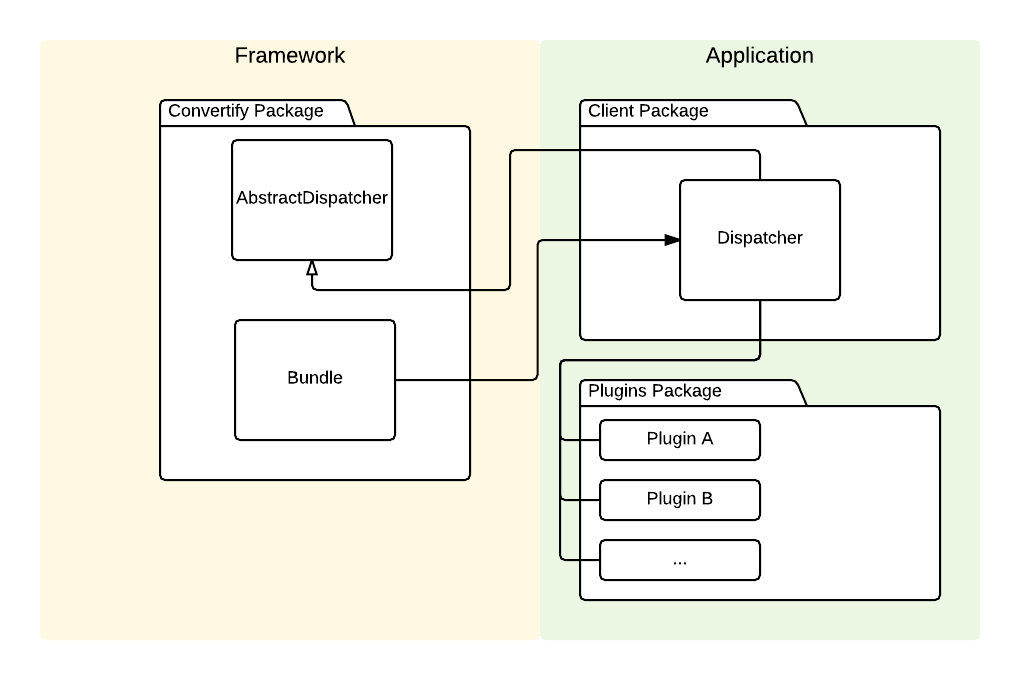
\includegraphics[width=1.1\columnwidth]{03-architecture-bundle-dispatcher}
  \caption{A \class{Bundle} is configured with a \class{Dispatcher}.}
  \label{fig:bundle-dispatcher}
\end{figure}

% whats a bundle
% bundle class

% have it for frontend/ backend package (because loading files etc. is different in browser/ nodejs)
% entry point, initialized with a dispatcher. dispatchers are written in application code.
% so convertify behavior configured via bundle through custom dispatcher.

% why have a bundle?

% give controller for convertify eco system, used by applications, e.g platener
% easy customization -> e.g. synching scenes of multiple instances of convertify -> animations/ controls/ loaded models


\subsection{{\convertify} is a cross-platform isomorphic framework}
\label{sec:convertify-is-isomorphic}

\note{explain crossplatform}
\note{same fro cross as for isomoprhic...}


\note{explain isomorphic = headless}
\note{explain what convertify can do when isomorphic}
\note{explain how convertify is isomorphic}
\note{explain why convertify is isomorphic (pros)}


\subsection{{\convertify} is built on {\brickify}}
\label{sec:brickify-comparison}

The web application {\brickify} was introduced in
Section~\ref{}\note{ref to related work}. {\brickify} provides several
features that we reuse for {\convertify}. We integrate the rendering
engine with its scene management and event system. We greatly improve
the event system by using a \class{Dispatcher}. Also, {\brickify}
provides the basic functionality of our plugin system. Though we
enhance plugin-plugin communication via \class{Protocols}. In general
{\brickify} combines UI-elements with its logic components. With
{\convertify}, we have a framework that is completely decoupled from
any user-interface code.

\subsection{A Variety of Possible Applications Can Be Built With the {\convertify} Architecture}
\label{sec:variety-of-applications}

Thanks to {\brickify}'s groundwork and our improvements to their
system, we cover a set of general functionality which is useful for
any web-based 3D application. We focus on 3D-Models as primary data
representation. We enable users to perform customization to these
models in real-time. The computed results are visualized for the user.
We support cross-platform browsers using WebGL technology. We allow
mouse and touch interactions with the scene. This enables users to
interact with {\convertify} from desktop or mobile systems.

\note{could be integrated in other applications when used headless,
  e.g. 3d editor for laser cutting}

\end{document}

%%% Local Variables:
%%% mode: latex
%%% TeX-master: "../../ClassicThesis"
%%% TeX-command-extra-options: "-shell-escape"
%%% End:
